\section{Usability-Studie BYU 2019}

\subsection*{Allgemeines}
\begin{frame}
    \frametitle{Usability-Studie BYU 2019}
    \begin{itemize}
        \item Brigham Young Universität, Utah
        \item 2 unabhängige Studien
        \begin{enumerate}
            \item zwei-wöchige Studie zur Nutzung der 2FA-Methode
            \item Studie zur Einrichtung der verschiedenen Methoden
        \end{enumerate}
        \item Betrachtung von Zeit und Gebrauchstauglichkeit
    \end{itemize}
    \note{
        \begin{itemize}
            \item Behandelte 2FA Methoden und Kontrollgruppe ohne 2FA
            \begin{itemize}
                \item SMS
                \item TOTP
            \end{itemize}
            \item keine `remember me`-Funktion, sodass immer zweiter Faktor benutzt werden musste
        \end{itemize}
    }
\end{frame}

\subsection{tagtägliche Nutzung}
\begin{frame}
    \frametitle{\currentsectionname}
    \begin{itemize}
        \item 73 Teilnehmer*innen
        \item 6 Gruppen \'{a} 12 Personen
        \item Einloggen in Online Banking-App
        \item Absolvieren von 12 Aufgaben innerhalb von zwei Wochen
        \item maximal eine Aufgabe pro Tag
    \end{itemize}
\end{frame}

\begin{frame}
    \frametitle{Authentifizierungszeit}

    \begin{itemize}
        \item Zeit von erfolgreicher Eingabe des Passworts bis Authentifizierung
    \end{itemize}

    % tabellarische Darstellung
    % \pgfplotstabletypeset[col sep=comma,
    %     columns/2FA-Methode/.style={string type},
    % ]{data/authentication-time.csv}

    \begin{figure}[c]
        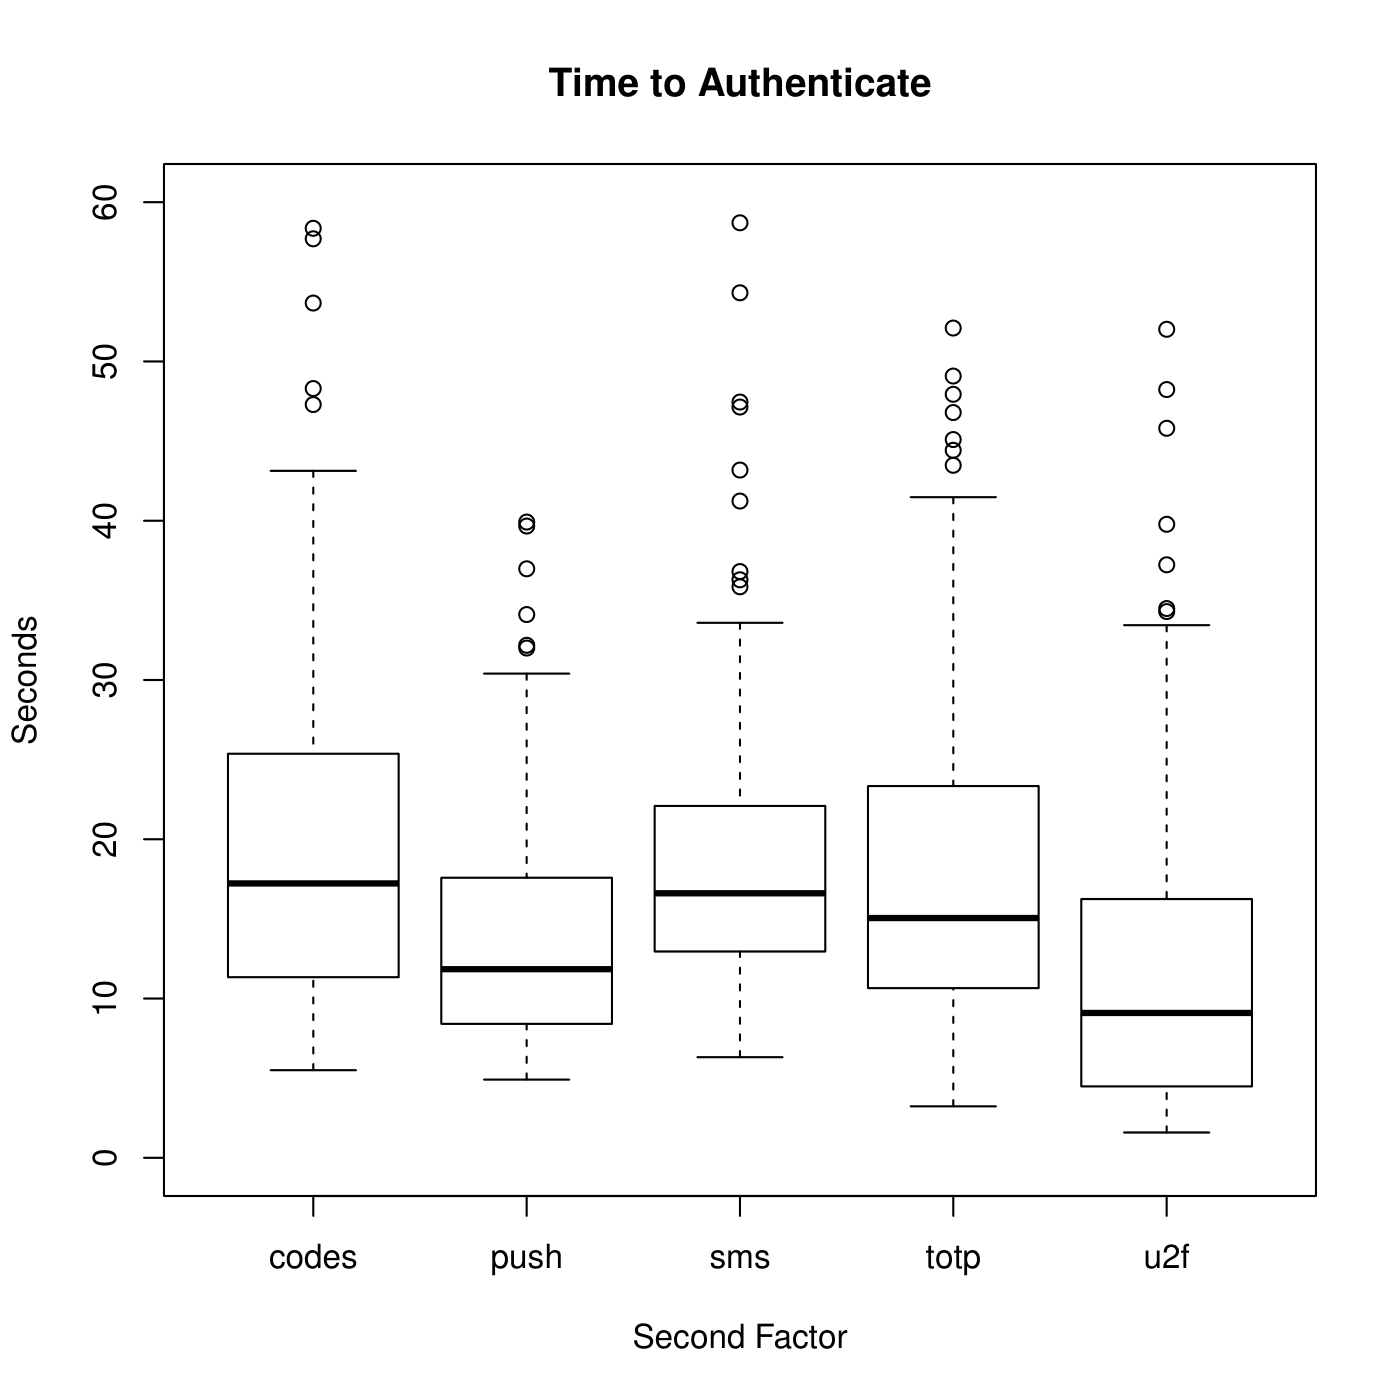
\includegraphics[height=0.8\textheight]{authentication-time}
        \(\nearrow \)\endnote{\cite{reese2019}}
    \end{figure}

\end{frame}

\begin{frame}
    \frametitle{Gebrauchstauglichkeit der Authentifizierung}

    \begin{itemize}
        \item Bewertung der wahrgenommenen Gebrauchstauglichkeit nach der Standardskala SUS\,
\includegraphics[height=0.25\baselineskip]{sus}
        \tiny{\textcolor{white}{\endnote{\url{https://borderpolar.com/wp-content/uploads/2021/06/red-among-us-png-842x1024.png.webp}}}}
    \end{itemize}

    \begin{figure}[c]
        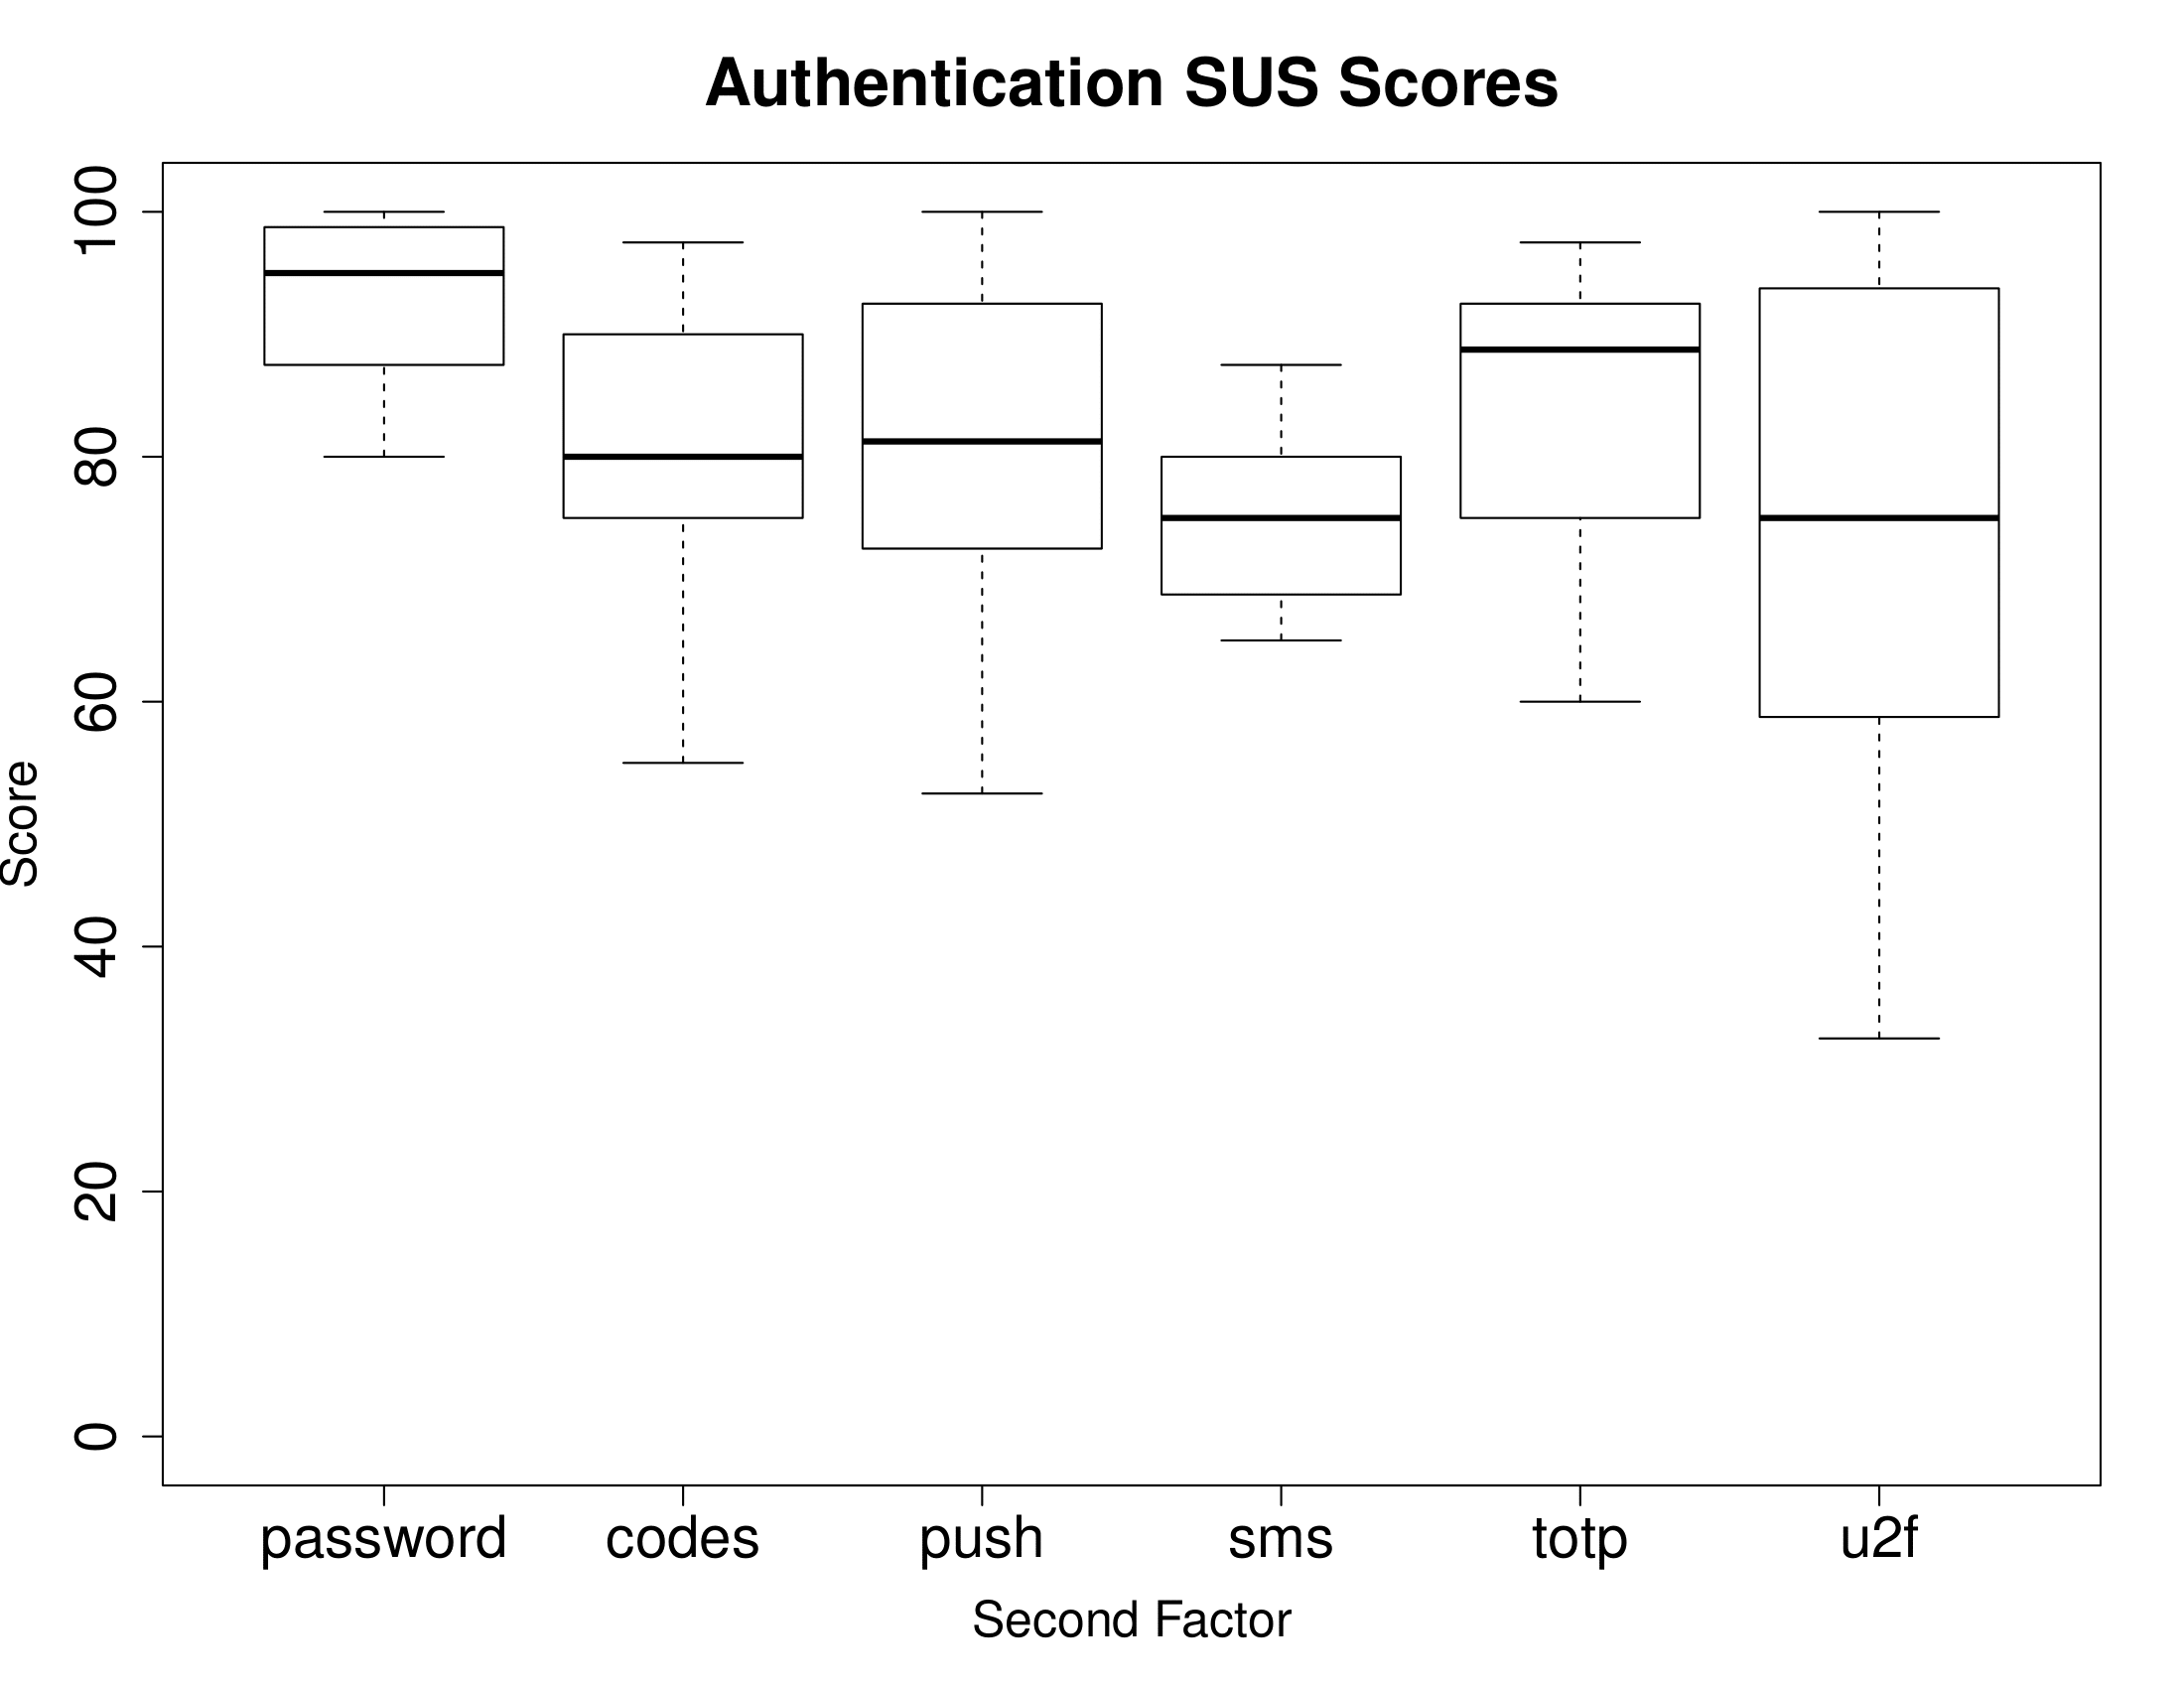
\includegraphics[height=0.8\textheight]{authentication-sus}
        \(\nearrow \)\endnote{\cite{reese2019}}
    \end{figure}

    \note{
        \begin{itemize}
            \item Passwort als Kontrollwert, andere Werte alle schlechter, fügen ja nur weitere Schritte hinzu
        \end{itemize}
    }

\end{frame}

\subsection{Einrichtung von 2FA}
\begin{frame}
    \frametitle{\currentsectionname}

    \begin{itemize}
        \item Einrichtung der fünf verschiedenen 2FA-Methoden wurde betrachtet
        \item gezielte getrennte Betrachtung von der generellen Gebrauchstauglichkeit
        \item 30 Teilnehmer*innen, welche jeweils jede Methode einrichten mussten
    \end{itemize}

\end{frame}

\begin{frame}
    \frametitle{Einrichtungszeit}
    \begin{itemize}
        \item Zeit zwischen Beginn der Einrichtungsaufgabe bis zur Fertigstellung
    \end{itemize}
    \begin{figure}[c]
        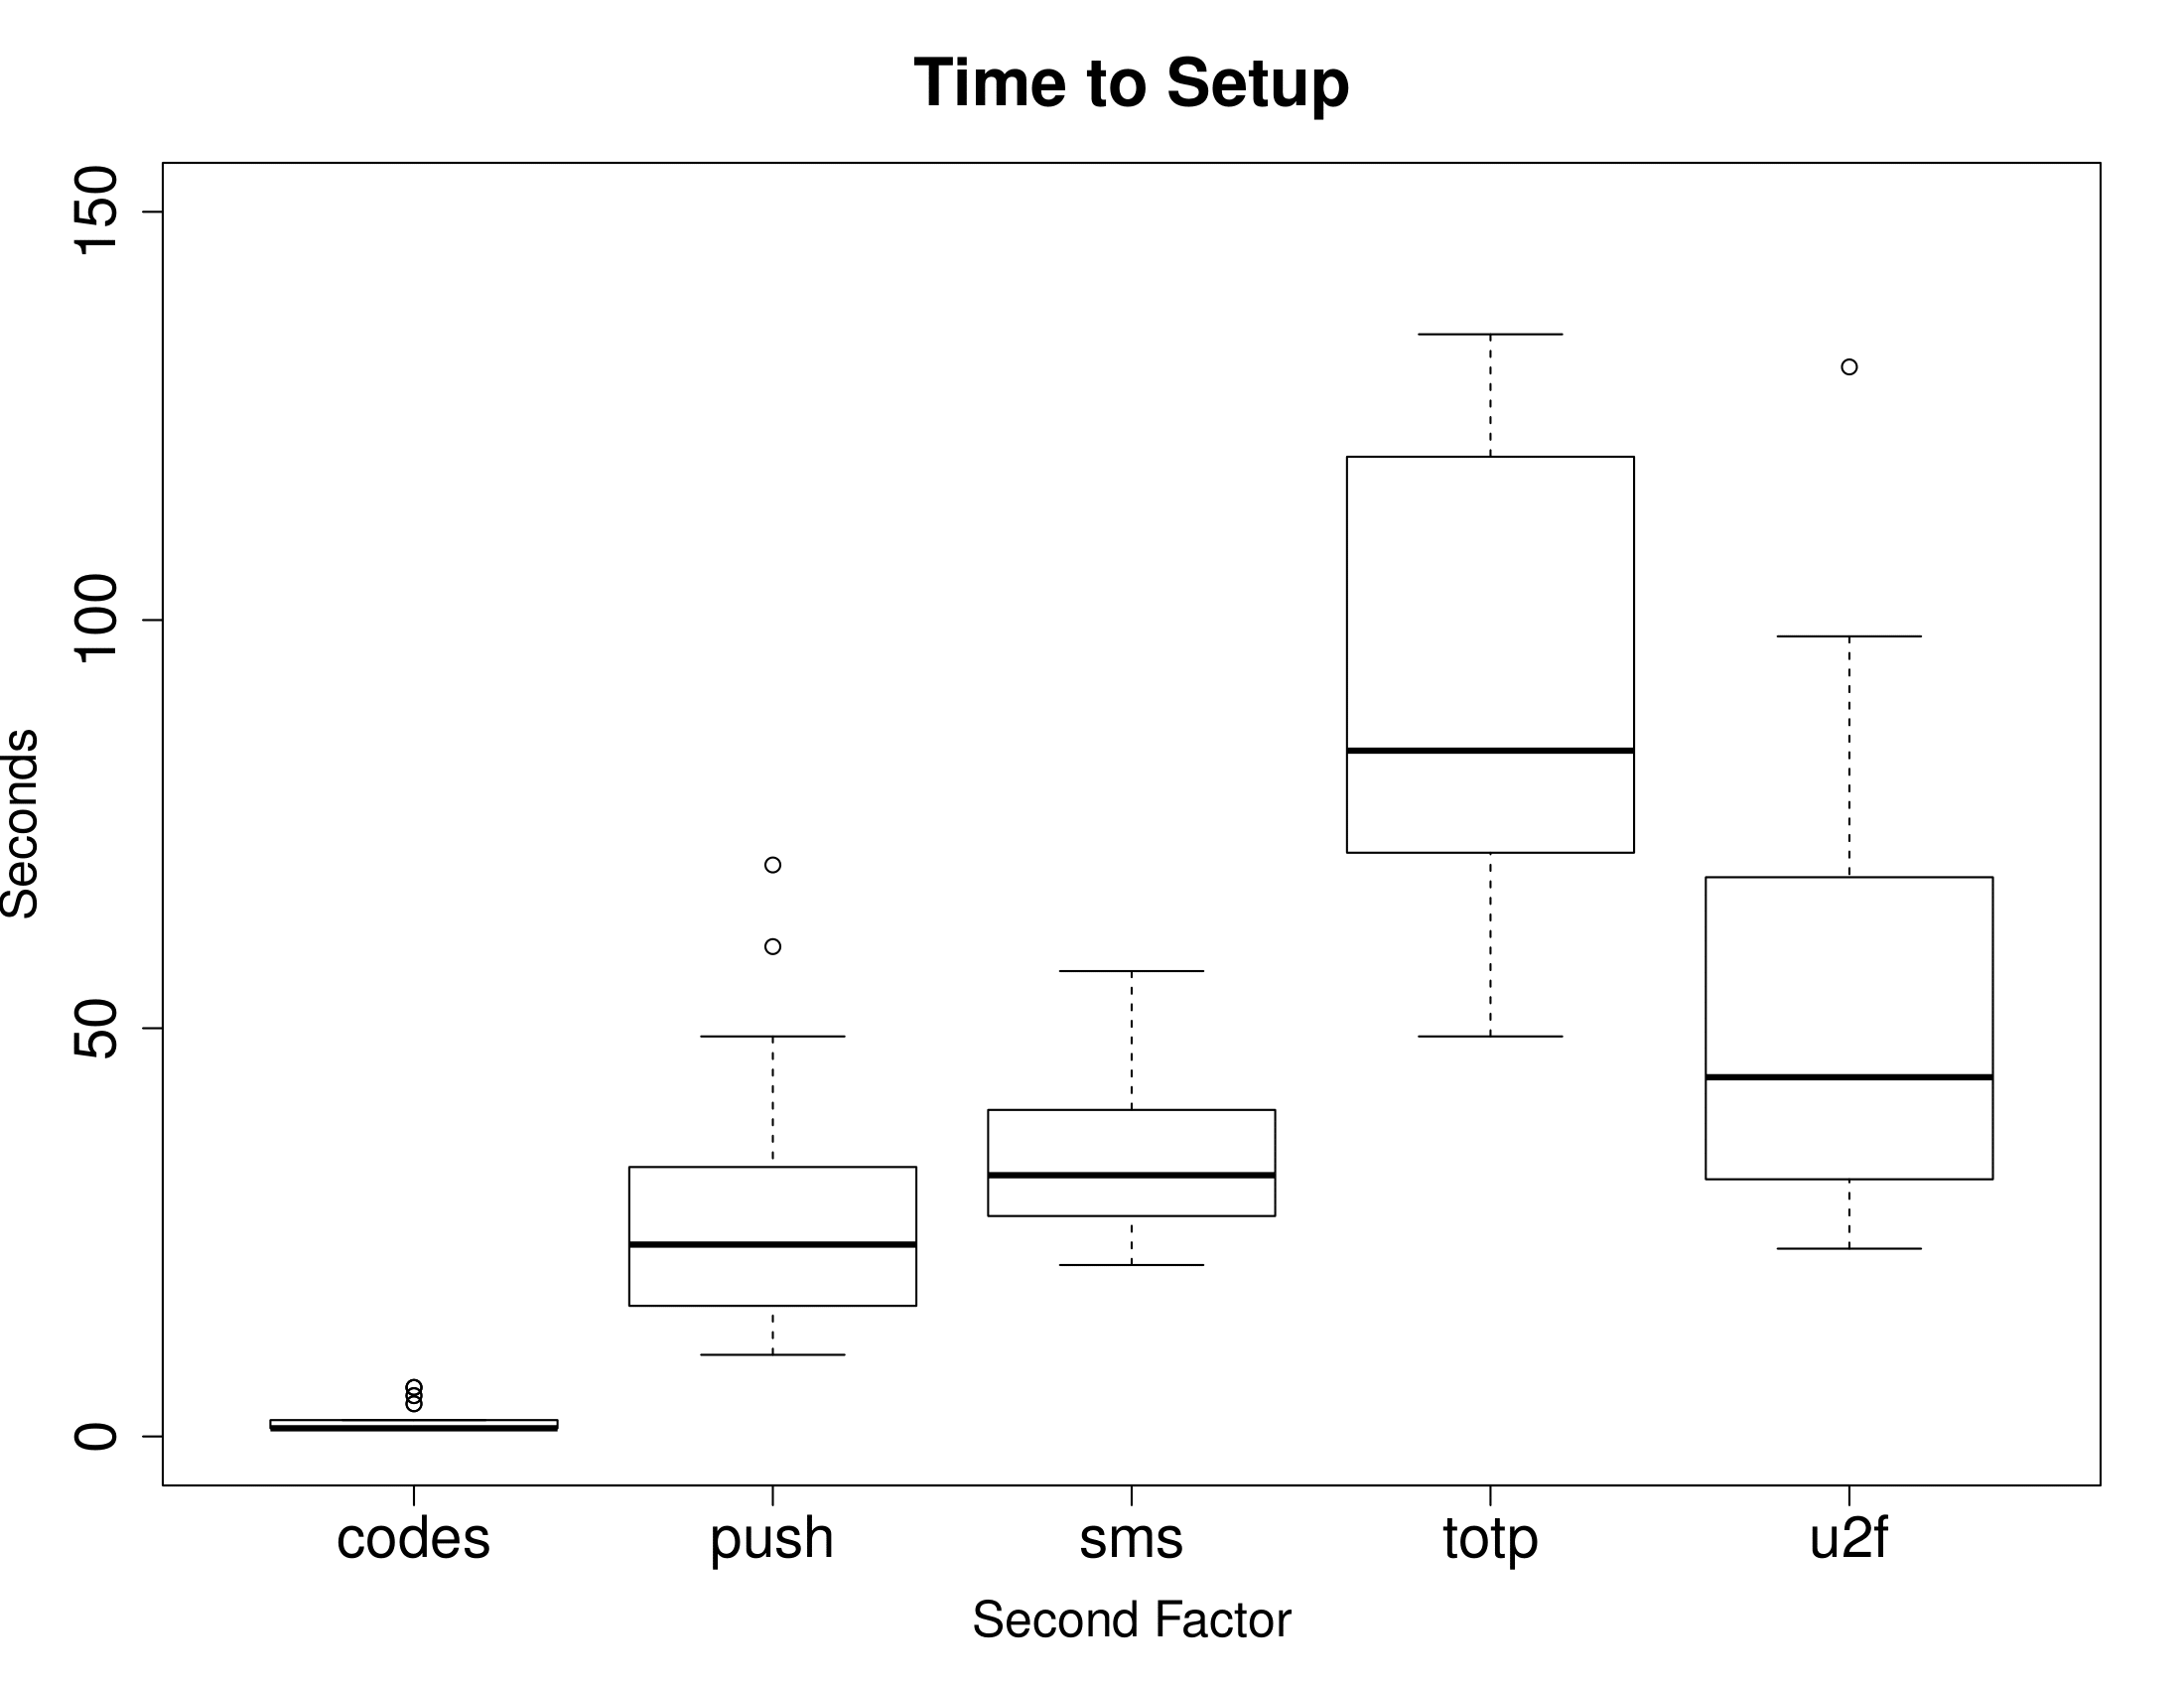
\includegraphics[height=0.8\textheight]{setup-time}
        \(\nearrow \)\endnote{\cite{reese2019}}
    \end{figure}

\end{frame}

\begin{frame}
    \frametitle{Gebrauchstauglichkeit der Einrichtung}

    \begin{itemize}
        \item Erfassung über Single Ease Question (SEQ), Skala von 1 bis 7
    \end{itemize}

    \begin{figure}[c]
        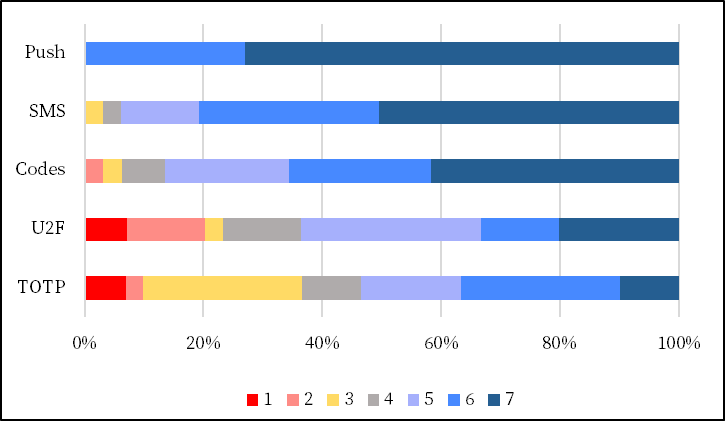
\includegraphics[height=0.7\textheight]{setup-seq}
        \(\nearrow \)\endnote{\cite{reese2019}}
    \end{figure}

\end{frame}

\subsection{Ausblicke und Vergleich mit anderen Studien}
\begin{frame}
    \frametitle{\currentsectionname}

\end{frame}
